\documentclass[border=6pt]{standalone}
\usepackage{amsmath}
\usepackage{tikz}
\usetikzlibrary{arrows.meta,decorations.pathreplacing}
\begin{document}
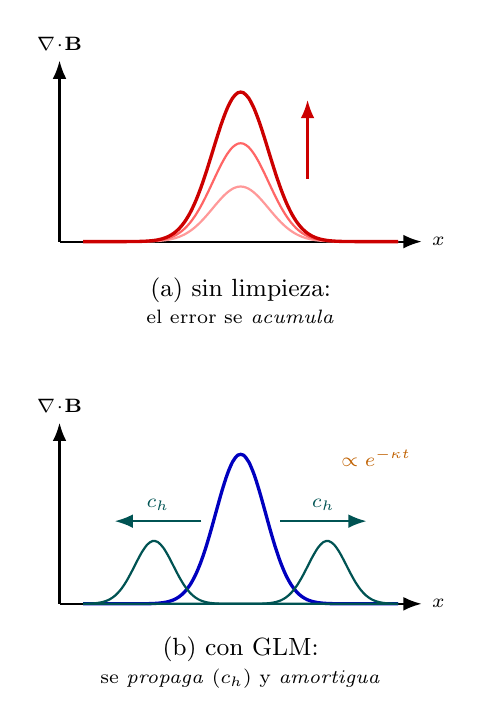
\begin{tikzpicture}[>=Latex,scale=1.0]

% ====== Panel A: sin GLM (el error se acumula) ======
\begin{scope}
  \draw[thick,->] (-2.3,0) -- (2.3,0) node[right,font=\scriptsize]{$x$};
  \draw[thick,->] (-2.3,0) -- (-2.3,2.3) node[above,font=\scriptsize]{$\nabla\!\cdot\!\mathbf B$};
  % pico que crece (3 curvas cada vez mayores)
  \draw[red!40,thick,smooth,samples=60,domain=-2:2] plot (\x,{0.7*exp(-(\x*\x)/0.25)});
  \draw[red!60,thick,smooth,samples=60,domain=-2:2] plot (\x,{1.25*exp(-(\x*\x)/0.25)});
  \draw[red!80!black,very thick,smooth,samples=60,domain=-2:2] plot (\x,{1.9*exp(-(\x*\x)/0.25)});
  \draw[->,red!80!black,thick] (0.85,0.8) -- (0.85,1.8);
  \node[font=\small,align=center] at (0,-0.75) {(a) sin limpieza:\\[-1pt]\scriptsize el error se \emph{acumula}};
\end{scope}

% ====== Panel B: con GLM (se propaga y amortigua) ======
% (ronda 3) apilado DEBAJO del panel A para ganar tamano vertical
\begin{scope}[yshift=-4.6cm]
  \draw[thick,->] (-2.3,0) -- (2.3,0) node[right,font=\scriptsize]{$x$};
  \draw[thick,->] (-2.3,0) -- (-2.3,2.3) node[above,font=\scriptsize]{$\nabla\!\cdot\!\mathbf B$};
  % pico inicial alto
  \draw[blue!75!black,very thick,smooth,samples=60,domain=-2:2] plot (\x,{1.9*exp(-(\x*\x)/0.2)});
  % dos pulsos que viajan hacia afuera y decaen
  \draw[teal!65!black,thick,smooth,samples=60,domain=-2:2] plot (\x,{0.8*exp(-((\x+1.1)*(\x+1.1))/0.12)});
  \draw[teal!65!black,thick,smooth,samples=60,domain=-2:2] plot (\x,{0.8*exp(-((\x-1.1)*(\x-1.1))/0.12)});
  % flechas de propagacion a c_h
  \draw[->,teal!65!black,thick] (-0.5,1.05) -- (-1.6,1.05) node[midway,above,font=\scriptsize]{$c_h$};
  \draw[->,teal!65!black,thick] (0.5,1.05) -- (1.6,1.05) node[midway,above,font=\scriptsize]{$c_h$};
  % decaimiento (arriba a la derecha, sin tocar los pulsos)
  \node[orange!75!black,font=\scriptsize] at (1.72,1.85) {$\propto e^{-\kappa t}$};
  \node[font=\small,align=center] at (0,-0.75) {(b) con GLM:\\[-1pt]\scriptsize se \emph{propaga} ($c_h$) y \emph{amortigua}};
\end{scope}

\end{tikzpicture}
\end{document}
